\documentclass[12pt]{mitthesis}
\usepackage{fullpage, braket, amsmath, amssymb}
\usepackage[pdftex]{graphicx}
\usepackage[version=3]{mhchem}
%\setlength{\parskip}{5mm}


\begin{document}

\section*{Delayed fluorescence measurements and intensity
  distributions in the frequency domain}

For a pure singlet bright state $\ket{s}$, the time-dependent
fluorescence intensity is
\begin{equation}
  I_s(t) = \frac{1}{\tau_s} \;
           \exp \left[
             -\frac{t}{ \tau_s} 
           \right],
\end{equation}
normalized such that $\int_0^{\infty} I_s(t) \, dt = 1$.

We consider the case where $\ket{s}$ is directly coupled with a set of
$N$ triplet dark states to create a set of $N$+1 mixed states
$\lbrace\ket{m}\rbrace$.  Each state $\ket{m}$ has some bright state
amplitude $a_m$.  In the case of direct or doorway-mediated coupling,
the Hamiltonian contains only one pathway from each dark state to the
bright state (see Chapter 3).  As a result, the mixing amlitudes may
be taken to be real and positive by convention.  If the lifetime of a
pure triplet dark state is much longer than $\tau_s$, the lifetime of
a mixed eigenstate $\ket{m}$ having bright state character
$\alpha_m^2$ is
\begin{equation}
  \label{eq:tau-m}
  \tau_m = \tau_s / a_m^2,
\end{equation}
and its time-dependent fluorescence intensity is
\begin{equation}
  \label{eq:int-m}
  I_m(t) = \frac{a_m^4}{\tau_s} \;
           \exp \left[
             -\frac{a_m^2 \, t}{\tau_s} 
           \right].
\end{equation}
The total integrated fluorescence intensity for a mixed state is
$\int_0^{\infty} I_m(t) \, dt = a_m^2$, relative to unit intensity for
a pure bright state.

The normalization condition for bright state character $\sum_m a_m^2 =
1$ leads to the relation
\begin{equation}
  \tau_s^{-1} = \sum_m \tau_m^{-1};
\end{equation}
in this way, $\tau_s$ can be derived from the set of mixed state
lifetimes $\lbrace \tau_m \rbrace$.



% \subsection*{Relation between average matrix element and average
%   lifetime}

% We wish to characterize the group of mixed states by their average
% fluorescence lifetime $\braket{\tau_m}$.  For the simple case of
% direct coupling to a group of evenly spaced levels, the bright state
% character follows a Lorentzian distribution in energy,  
% \begin{equation}
%   a_m(E) = 
%     \frac{1}{\pi} 
%     \frac{\Gamma/2}{(E-E_s)^2+(\Gamma/2)^2}.
% \end{equation}
% The width is given by the golden rule relation
% \begin{equation}
%   \Gamma = 2 \pi \braket{H_{m}^2} \rho_m.
% \end{equation}
% The average bright state character within the FWHM of the distribution
% is
% \begin{equation}
%   \label{eq:avg-char}
%   \braket{a_m^2}_{FWHM} = \frac{1}{2 \Gamma}.
% \end{equation}
% Combining equations \ref{eq:avg-char} and \ref{eq:tau-m}, we have
% \begin{equation}
%   \braket{\tau_m}_{FWHM} = 2 \Gamma \tau_s = 4 \pi \braket{H_{m}^2} \rho_m \tau_s.
% \end{equation}
% We have derived, for the simplest case, a proportional relationship
% between the average matrix element and average lifetime of a
% set of mixed states $\lbrace\ket{m}\rbrace$.


\subsection*{SEELEM detection as an extreme limit of delayed fluorescence}

We examine the fluorescence intensity after a time delay $t_c$,
which we cast in units of the bright state lifetime:
\begin{equation}
  R_c = t_c / \tau_s.
\end{equation}
At a chosen $R_c$, the fluorescence intensity equation has a single
peak according to some value of bright state character.  Within the
range $0 \le a_m^2 \le 1$, the fluorescence intensity equation is at a
maximum when (Chapter 2, equation 31)
\begin{equation}
  \label{eq:am-max}
  a_m^2 = \frac{2}{R_c}.
\end{equation}

\begin{figure}
  \caption{The intensity of a mixed eigenstate at time $R_c =
    t/\tau_s$, plotted as a function of bright
    state character.}
  \label{fig:int-at-rc}
  \centering
  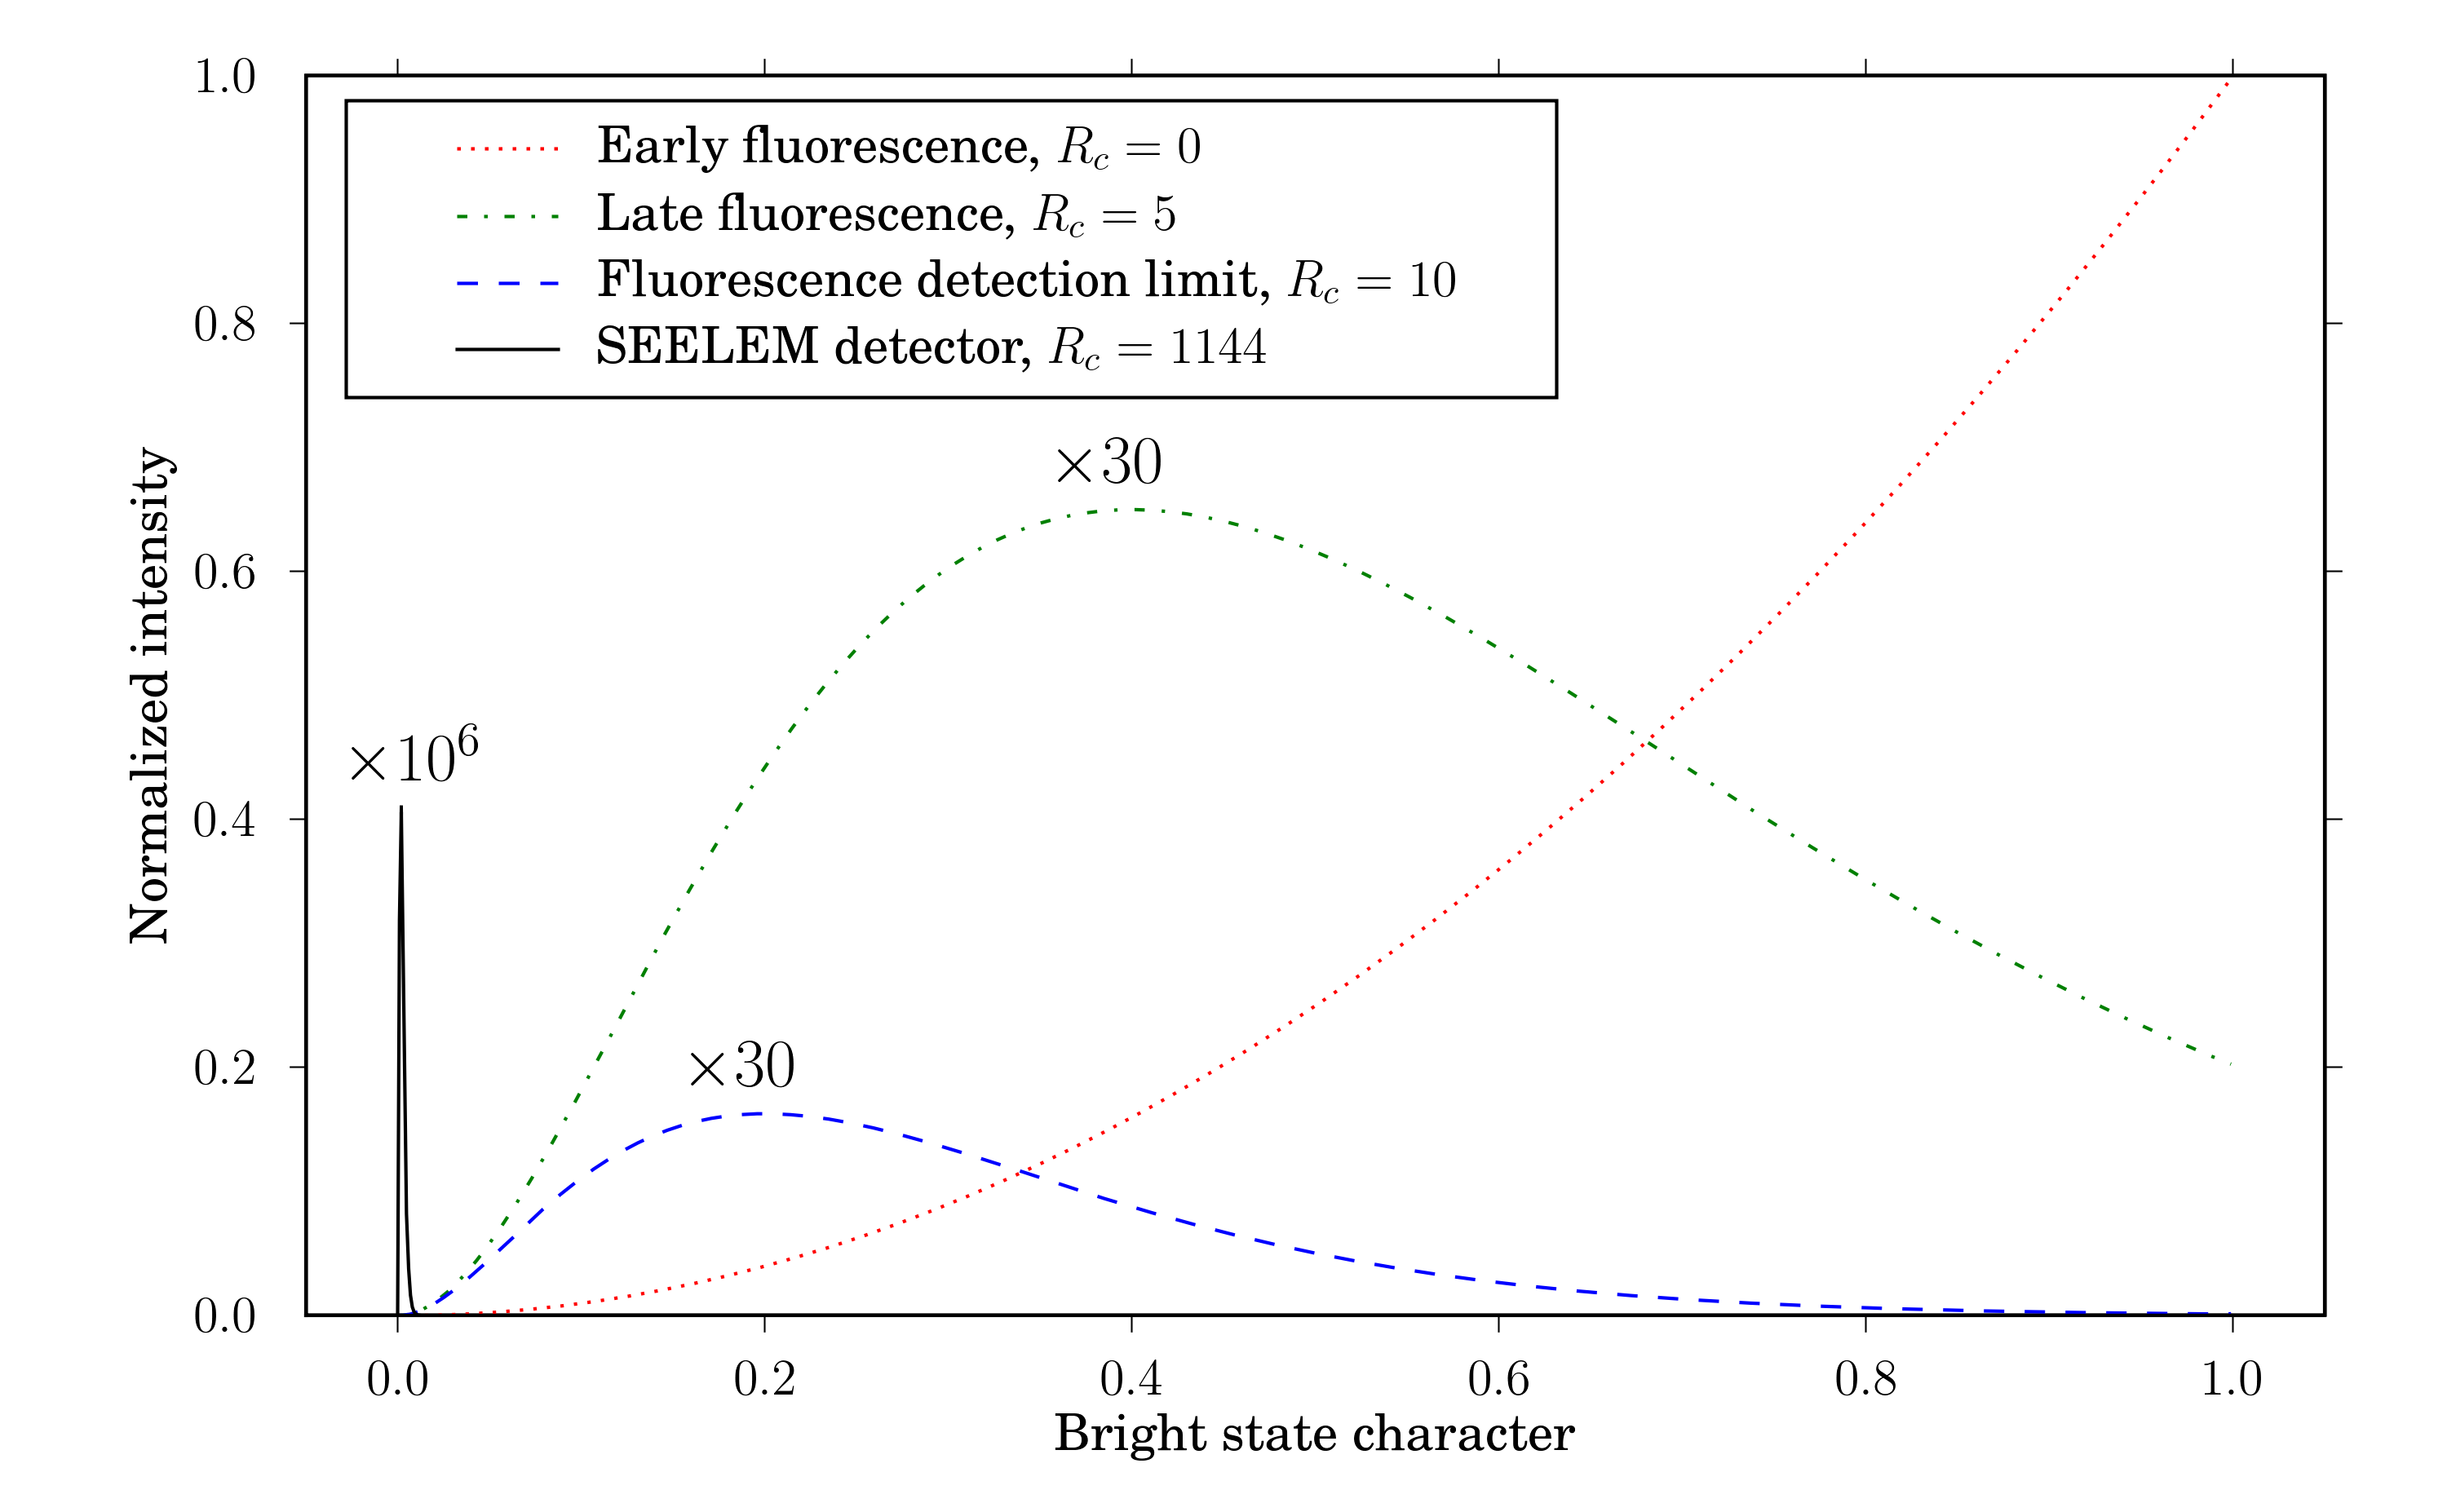
\includegraphics[width=6.7in]{intensity-at-rc.png}
\end{figure}

Figure \ref{fig:int-at-rc} shows the dependence of fluorescence
intensity on bright state character for several values of $R_c$.  At
early fluorescence times ($\sim \tau_s$), the fluorescence intensity
is greatest for states with large amounts of bright state character
($2/R_c > 1$).  At a delay of $5 \tau_s$, the fluorescence intensity
equation discriminates against states with large amounts of bright
state character, since molecules in such states have already
fluoresced with high probability.  States with small amounts of bright
state character are also discriminated against -- molecules in these
states have a low probability of fluorescing at the time under
consideration.  The fluorescence intensity is thus ``tuned'' to a
particular value of bright state character at every time delay $R_c$,
according to Equation \ref{eq:am-max}.

Note that the intensity expression used here does not account for
molecules leaving the field of view of the fluorescence detection
optics.  We consider only the distribution of bright state character
\emph{among molecules remaining in the field of view at time $R_c$}.
However, since there is no momentum transfer from the excitation
photon to the molecule, the rate of molecules exiting the field of
view is independent of bright state character.  Therefore,
simple reasoning according to the above intensity formulas will be
correct as long as we discuss fluorescence intensities only in terms
of ratios.

To foster a more concrete discussion, consider our experiments on
intersystem crossing in acetylene.  For the $S_1$ electronic state,
$\tau_s=270$ ns.  In our apparatus, the field-of-view of the
fluorescence detection optics is several mm, which amounts to a
maximum viewing time of 3 $\mu$s, about $10\tau_s$, for molecules in
the molecular beam with a velocity of $10^3$ m/s.  At times later than
$10\tau_s$, there are simply no molecules left to observe in the
fluorescence field of view.  This places an upper limit on the value
of $R_c$ that can be examined in our fluorescence experiments.  Figure
\ref{fig:int-at-rc} shows the intensity equation for the limit of
fluorescence detection, $10\tau_s$.

The SEELEM detector used in our experiments detects metastable
molecules after a 309 $\mu$s flight time.  If we set aside some
particularly interesting aspects of SEELEM detectivity and consider
only its detection sensitivity to bright state character, we arrive at
the following equation for SEELEM detection probability (Chapter 2,
equation 28):
\begin{equation}
  \label{eq:seelem-prob-s}
  P_{SEELEM}^{(s)} \propto a_m^4 \; \exp \left( -R_c \, a_m^2 \right).
\end{equation}
(This is a good approximation to its overall detection sensitivity,
including $T_3$, in the weak coupling limit.)  The SEELEM detection
probability equation above has the same functional form as the
Equation \ref{eq:int-m}.  Thus, the SEELEM detector may be viewed in
this limited sense as an extreme discriminator for states with small
amounts of bright state character.

Acetylene molecules in our apparatus are detected after an average
flight time of 309 $\mu$s, yielding an $R_c$ value of $1144$ for the
SEELEM detector.  This corresponds to a maximum detection probability
for states with $0.17\%$ bright state character.  

% At a multiple $R_c$ of the bright state lifetime, the intensity ratio
% between a mixed state and the (hypothetical) pure bright state is
% \begin{equation}
%   \frac{I_m}{I_s} = a_m^4 \; 
%                    exp\left[
%                      R_c \, (1 - a_m^2)
%                    \right].
% \end{equation}
% This quantity reflects, at time $R_c$, the extent to which the
% experiment is discriminating in favor of a mixed eigenstate.  Figure
% \ref{fig:discr} shows a plot of $I_m/I_s$ as a function of $R_c$ for
% several values of bright state character.  States with bright
% character of 10\% become twice as intense as a pure bright state after
% $3\tau_s$.  For a mixed state with 1\% bright character, one must wait
% almost $5\tau_s$ before the discrimination factor increases to 1.

% \begin{figure}
%   \caption{The intensity of a mixed eigenstate relative to the
%     intensity of a pure bright state, as a function of time (units of
%     bright state lifetime $\tau_s$).  The bright state character
%     $a_m^2$ is varied from 1 to 20 percent.}
%   \label{fig:discr}
%   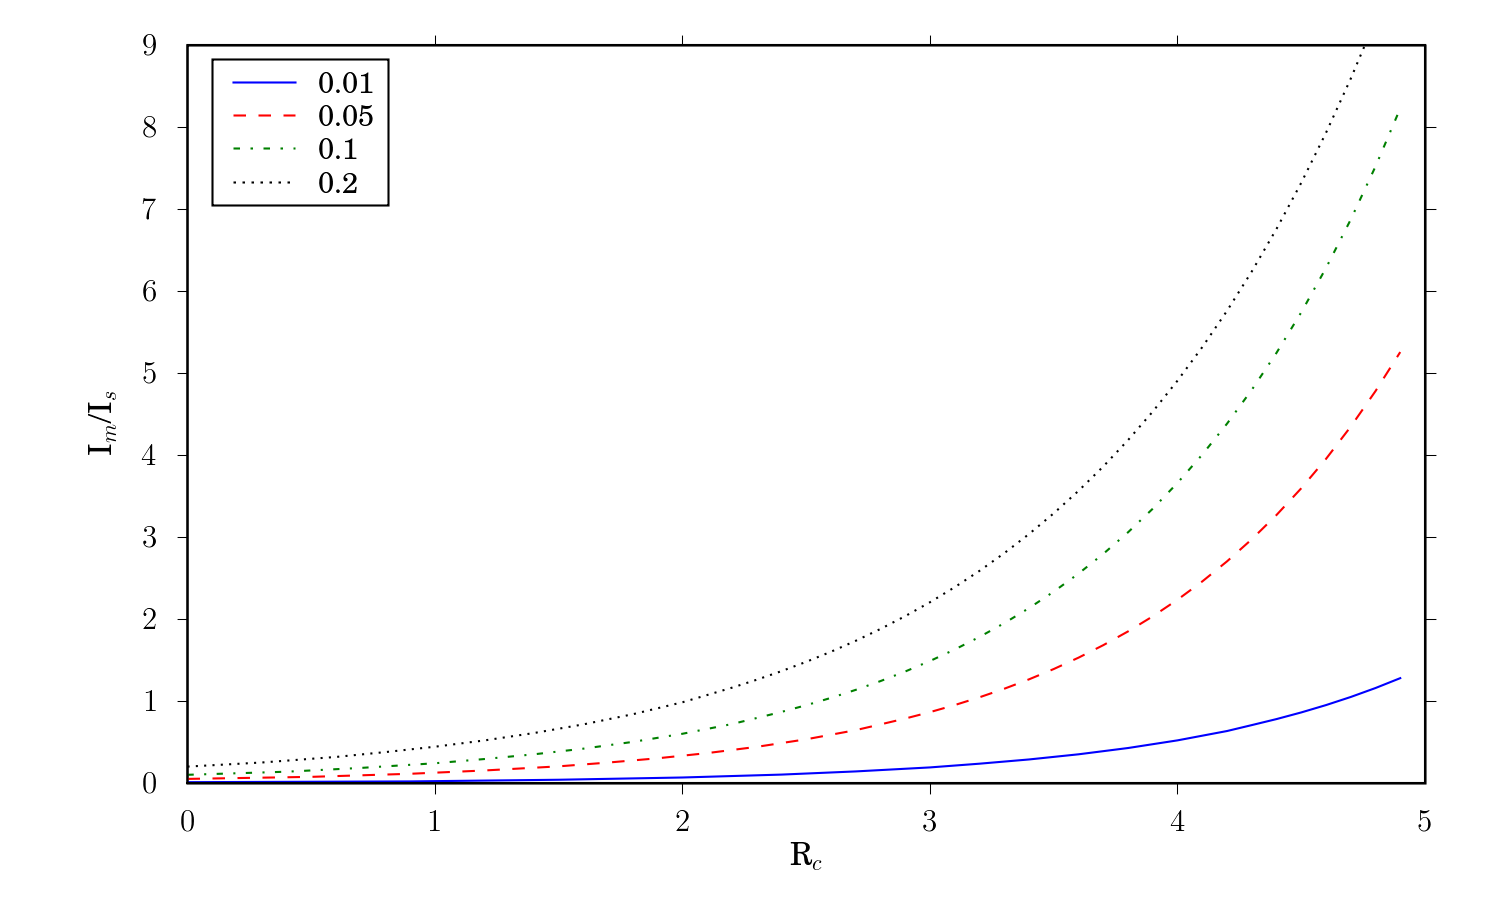
\includegraphics[width=6.5in]{longlife-discrimination.png}
% \end{figure}

% Fluorescing states are unobservable in an experiment if the detector
% noise exceeds the fluorescence intensity.  We discuss the noise in an
% experiment as a fraction $f_{\text{noise}}$ of pure bright state
% intensity at $t=0$.  A fluorescing state $\ket{m}$ becomes
% unobservable when
% \begin{equation}
%   I_m(t) = \frac{f_{\text{noise}}}{\tau_s}
% \end{equation}
% The delay time at which any state becomes undetectable is simply a
% function of the bright state character $a_m^2$:
% \begin{equation}
%   (R_c)_{\text{max}} = -\frac{1}{a_m^2} \; 
%                    log\left[
%                      \frac{f_{\text{noise}}}{a_m^2}
%                    \right].
% \end{equation}

\subsection*{Delayed fluorescence of a two-level system}

Our next step is to examine the changing characteristics of a
fluorescence intensity distribution as we increase the time delay
$R_c$.  We model the interaction between a bright state and an
ensemble of dark states by generalizing from a two-level system.
Consider a Hamiltonian with only one dark state.  Define the two mixed
states $\ket{m=1,2}$ as
\begin{equation}
  \begin{split}
    \ket{1} &=  (1 - \alpha^2)^{1/2} \ket{s} + \alpha \ket{t}\\
    \ket{2} &= -\alpha \ket{s} + (1 - \alpha^2)^{1/2} \ket{t}.
  \end{split}
\end{equation}
The fluorescence intensity of both states, relative to a pure bright
state, is
\begin{equation}
  \begin{split}
    I_1 &= \frac{(1 - \alpha^2)^2}{\tau_s} \; \exp 
          \left[
            - R_c \, (1 - \alpha^2)
          \right]\\
    I_2 &= \frac{\alpha^4}{\tau_s} \; \exp 
          \left[
            - R_c \, \alpha^2
          \right],
  \end{split}
\end{equation}
and the ratio of the fluorescence intensities changes with time as
\begin{equation}
  I_{12} = I_1 / I_2 = 
  \left(
    \frac{(1 - \alpha^2)}{\alpha^2}
  \right)^2
  \exp
  \left[
    - R_c \, (1 - 2\alpha^2)
  \right].
\end{equation}
The fluorescence intensity ratio may be used to write an equation for
the dependence of average intensity on $R_c$.
\begin{equation}
  \label{eq:ratio}
  \braket{I_{LIF}} = 
  \frac{\Delta E_{12}}{2} \,
  \left(
    \frac{I_{12}-1}{I_{12}+1}
  \right)
\end{equation}
Figure \ref{fig:ratio} shows the dependence of center-of-gravity on
the intensity ratio $I_{12}$.

\begin{figure}
  \caption{Center of gravity as a function of the intensity ratio
    $I_1$:$I_2$ for a two-state system.  At $t=0$, the initial center
    of gravity is a function of the mixing amplitude $\alpha$.  The
    center of gravity then shifts with the changing intensity ratio as
    delay time is increased, arriving at a limiting value of $-\Delta
    E_{12}/2$.}
  \label{fig:ratio}
  \centering
  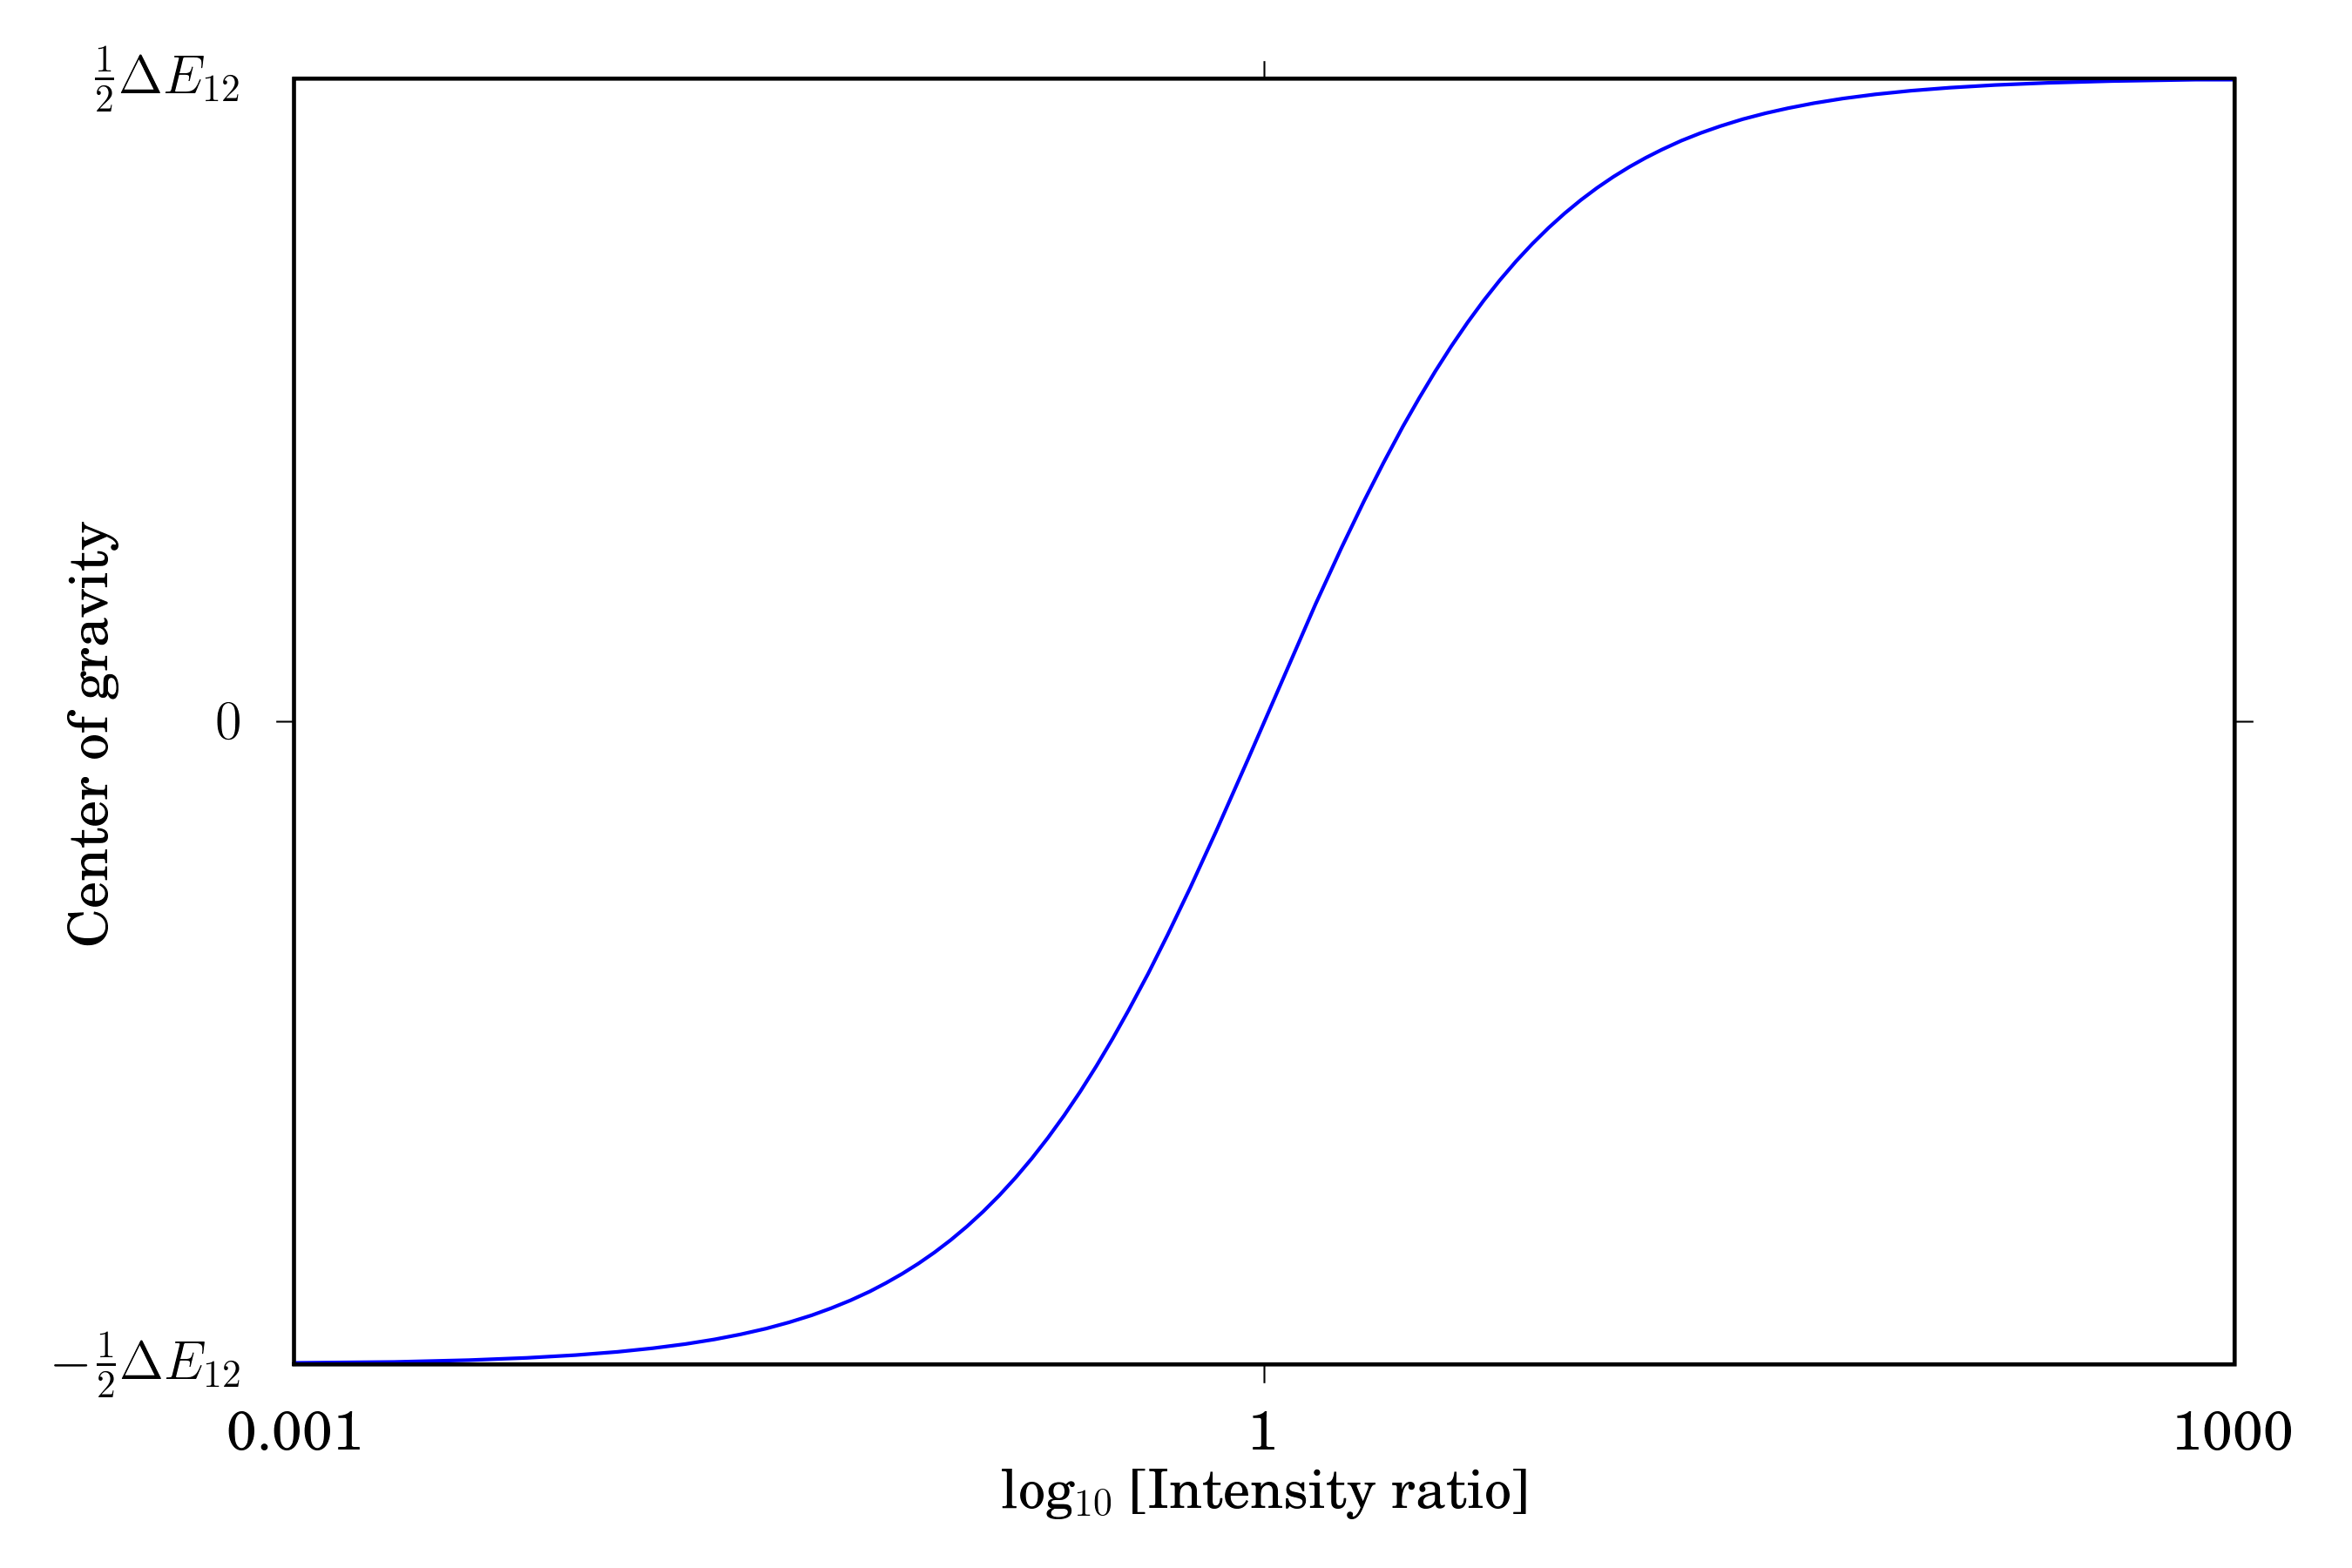
\includegraphics[width=6in]{cog-from-ratio.png}
\end{figure}

The initial intensity ratio at time $R_c=0$ is just
\begin{equation}
  I_{12} = 
  \left(
    \frac{(1 - \alpha^2)}{\alpha^2}
  \right)^2.
\end{equation}
From this, the initial center of gravity can be found according to
Equation \ref{eq:ratio} or Figure \ref{fig:ratio}.  At large values of
$R_c$, the intensity ratio decreases to zero as $I_1 \ll I_2$, as long
as the states are not 50:50 mixed.  As the ratio decreases to zero,
the center of gravity approaches $-\Delta E_{12} / 2$.  The
development of intensity ratios and the consequent shift in center of
gravity are shown in Figure \ref{fig:cog-devel}.  One interesting
aspect of the center of gravity shift shown in the figure is the rapid
onset of the shift at small mixing coefficients.  

\begin{figure}
  \caption{(Top) Time development of the relative intensity ratio for
    a two state system. (Bottom) Time development of the center of
    gravity for a two state system.}
  \label{fig:cog-devel}
  \centering
  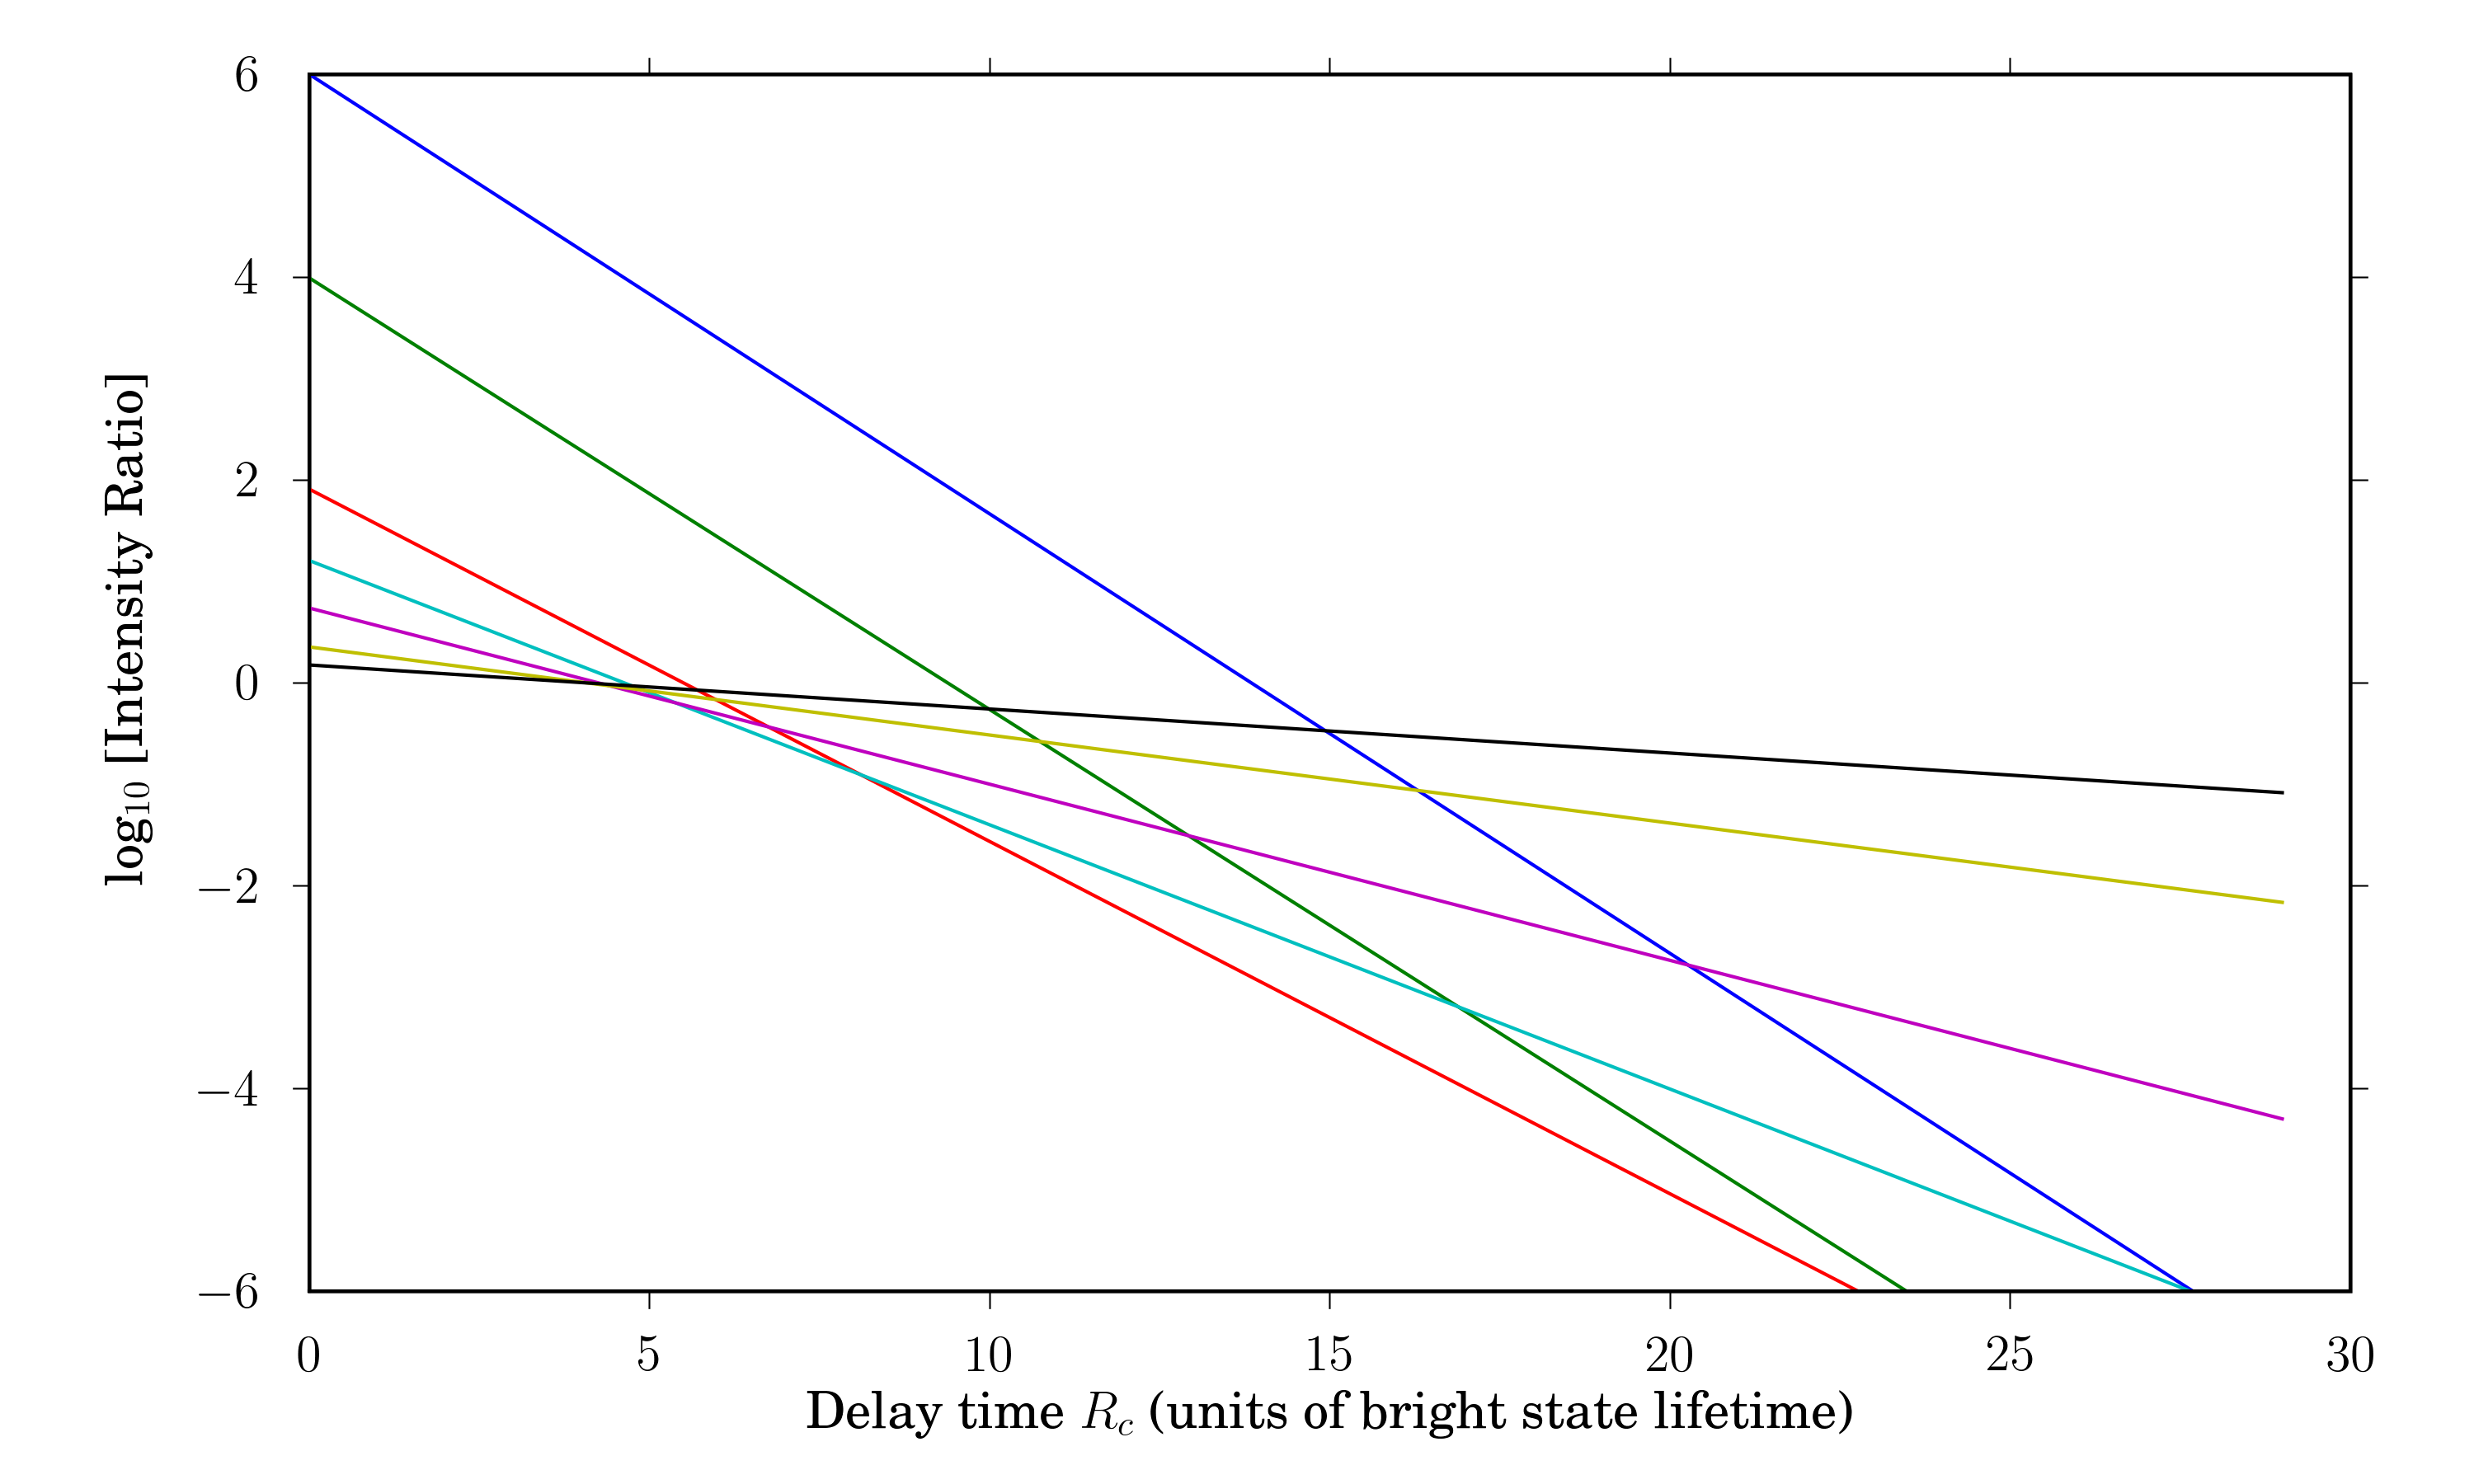
\includegraphics[width=6in]{ratio-development.png}
  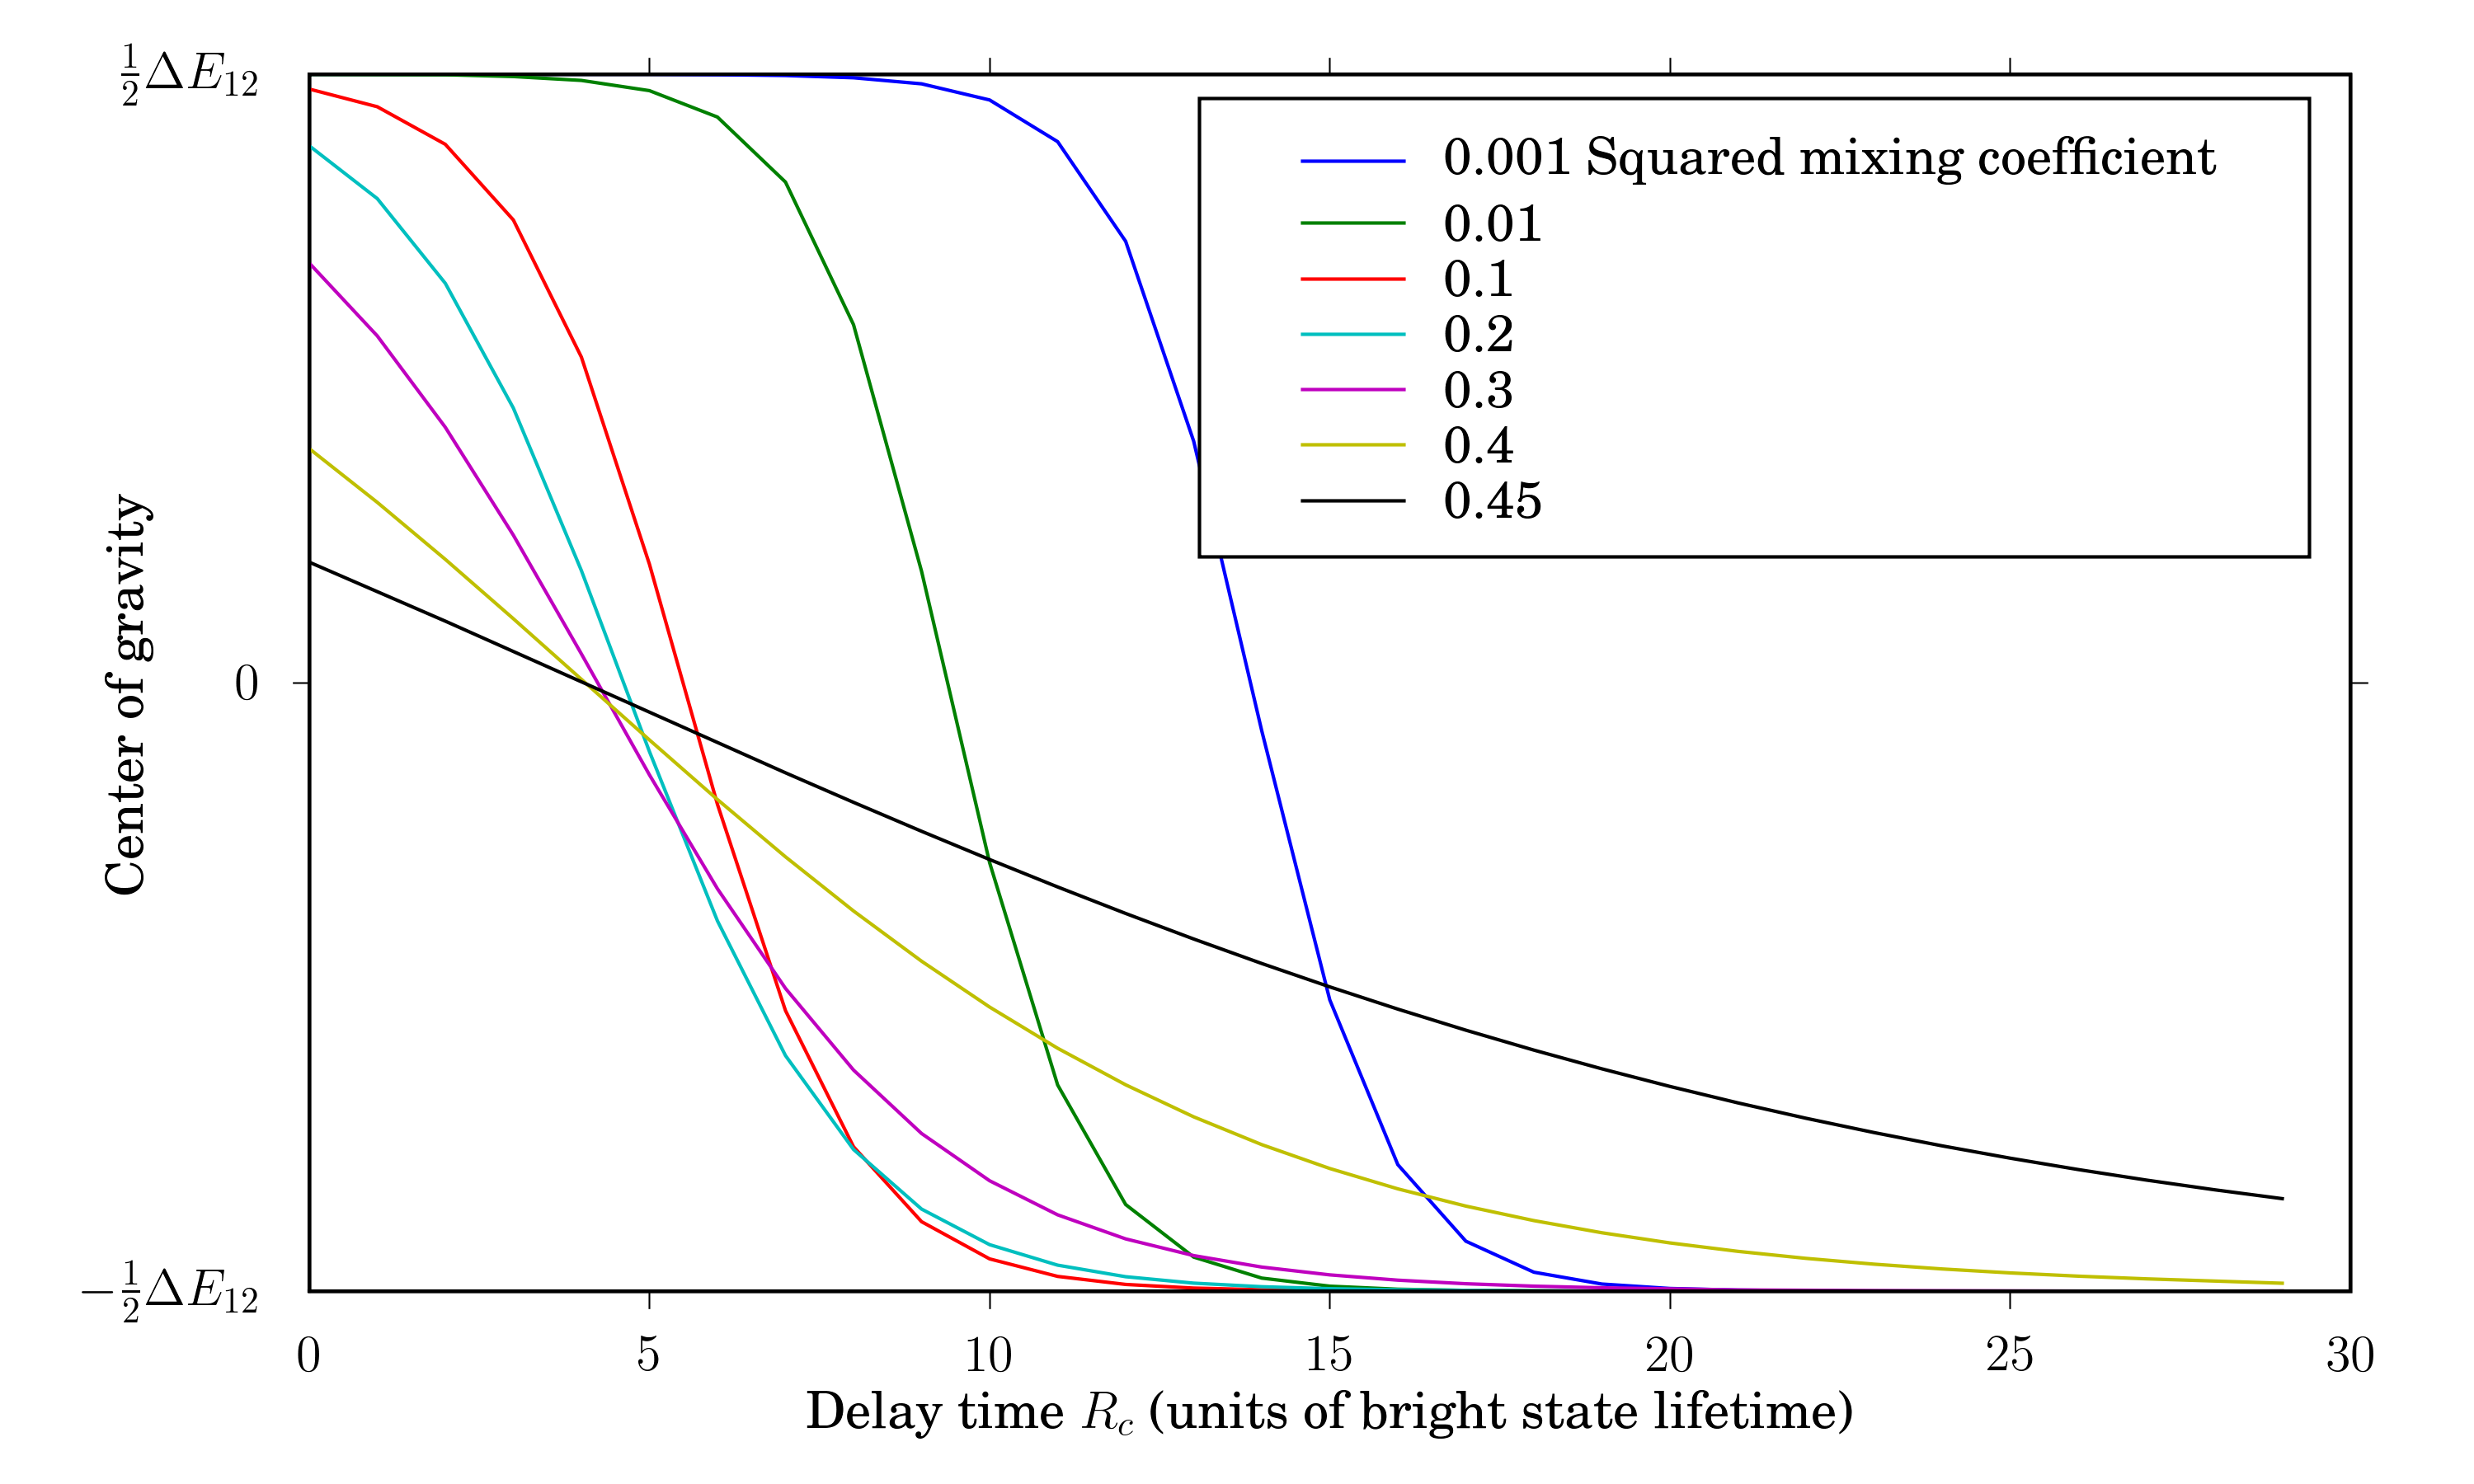
\includegraphics[width=6in]{cog-development.png}
\end{figure}

% We generalize this two-state treatment to larger systems by dividing
% the states of the system into two groups, according to the dynamics we
% wish to study.  The division may be made



\subsection*{Delayed fluorescence of several transitions}

Information about the relative B-value of a mediating level can be
recovered by studying the statistical properties of delayed
fluorescence as a function of rotational quantum number.

We take as a model system a series of equally spaced bright state
transitions with increasing rotational quantum number $J$.  The total
bright$\sim$dark coupling strength for each transition is function of
the energy separation between the bright state $\ket{s;J}$ and three
components of the non-local mediating level: $F_1$, $\ket{\ell;J-1}$;
$F_2$, $\ket{\ell;J}$; and $F_3$, $\ket{\ell;J+1}$.

The rotational dependence of energy differences for the three
components is
\begin{equation}
  \Delta E_{s\ell}(J) = 
  \begin{cases}
    \Delta B_{s\ell}J(J+1) + 2B_{\ell}J           & F_1 \text{ component}\\
    \Delta B_{s\ell}J(J+1)                      & F_2 \text{ component}\\
    \Delta B_{s\ell}J(J+1) - 2B_{\ell}J - 2B_{\ell} & F_3 \text{ component}.\\
  \end{cases}
\end{equation}
We simplify the above formulas by considering the \emph{average}
energy difference, taking all components into account.  Giving equal
weights to all components, the average energy separation is
\begin{equation}
  \Delta E_{s\ell}(J)_{\text{ave}} = \Delta B_{s\ell}J(J+1) - \frac{2}{3}B_{\ell}.
\end{equation}
We define a mixing coefficient $\alpha_{s\ell}$ between the bright
state and the three components of the mediating level.  The mixing
coefficient can be related to $\Delta E_{s\ell}$ using second order
perturbation theory.  Introducing the average spin-orbit matrix
element $H_{s\ell}$ for the three rotational components, the relation
is $\alpha_{s\ell}(J) = H_{s\ell} / \Delta E_{s\ell}(J)$.  The
relative strengths of the three components are given by simple
formulas, which can be found in the literature.  We find that the
functional dependence of the mixing coefficient between the bright
state and the mediating components is
\begin{equation}
  \alpha_{s\ell}(J) = \frac{H_{s\ell}}{\Delta B_{s\ell}J(J+1)}.
\end{equation}


\end{document}